\begin{figure}[htbp]
  \centering
  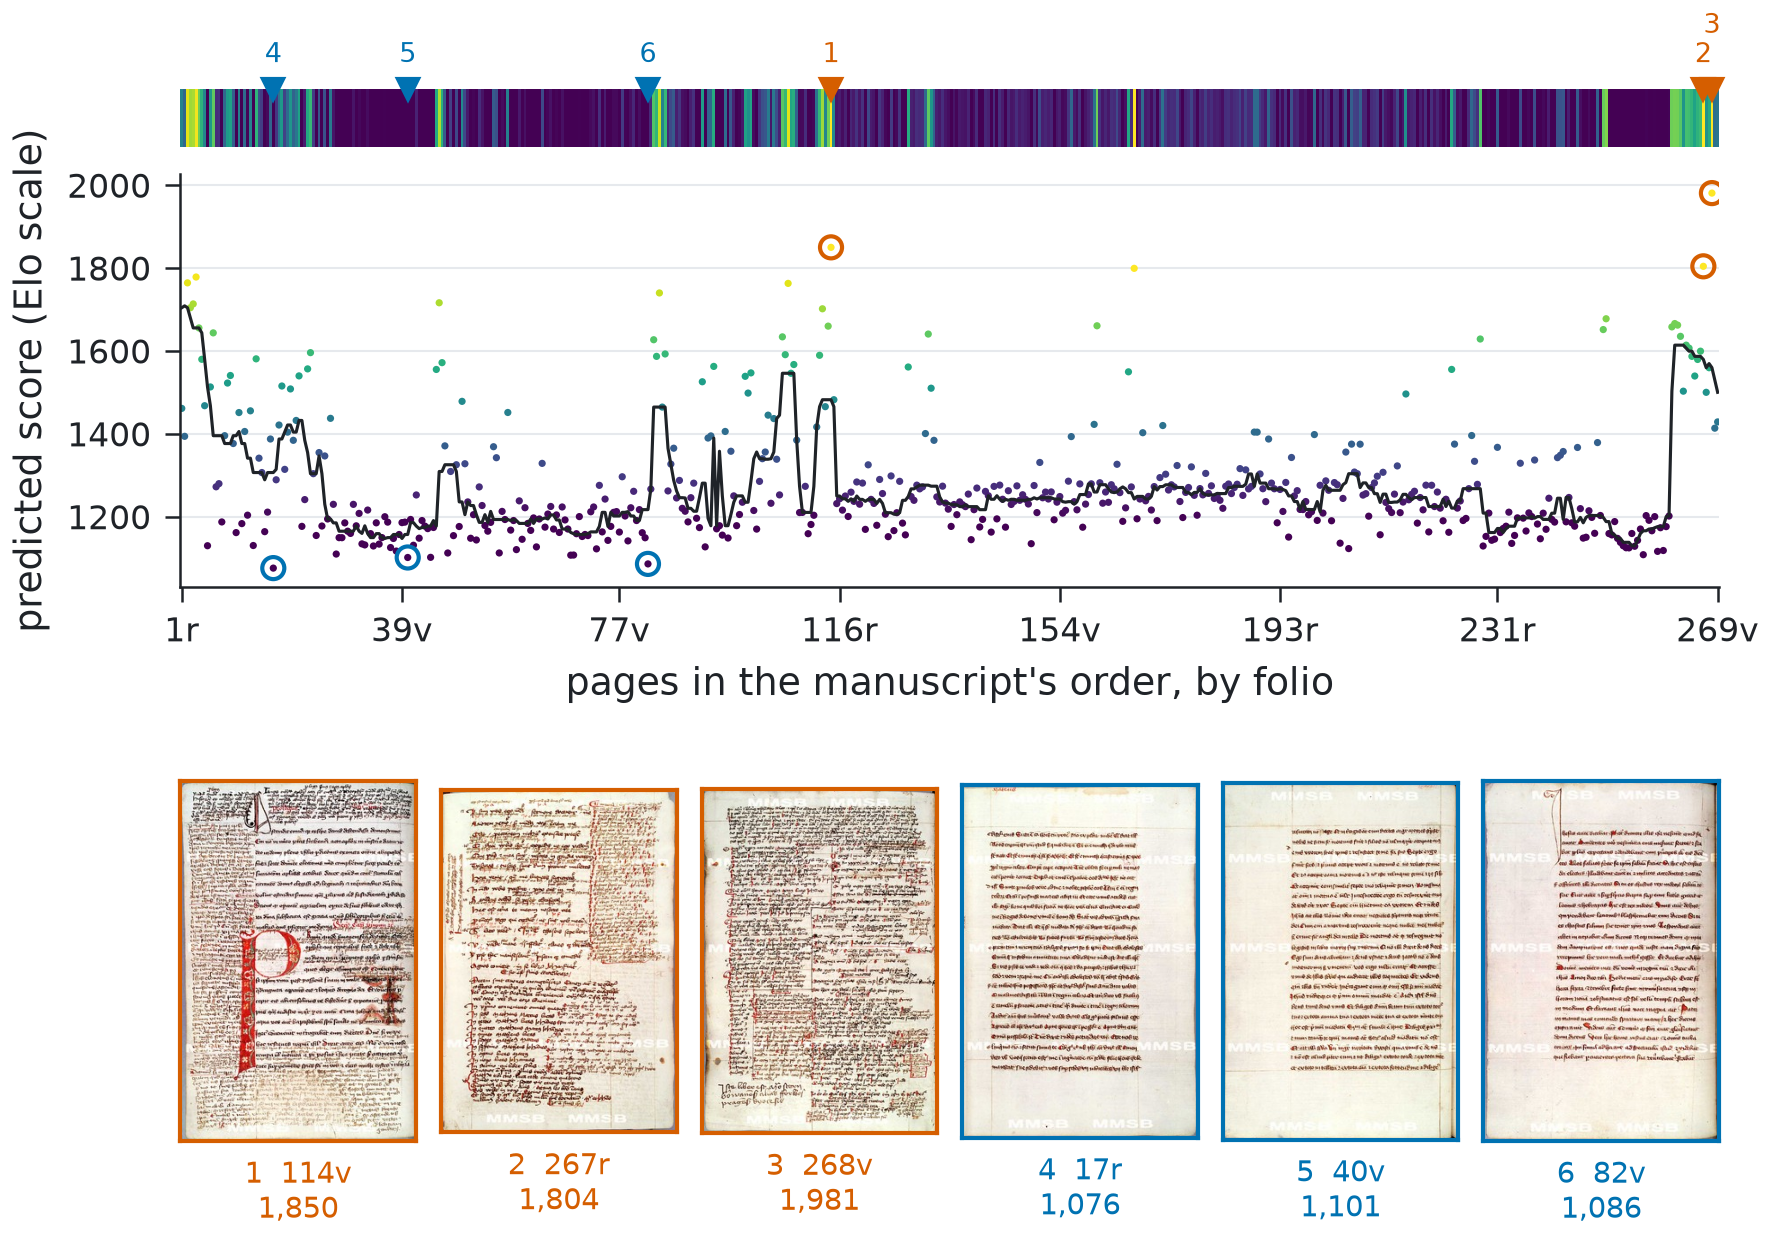
\includegraphics[width=15.00cm]{figures/manuscript_profile_id18.png}
  \caption{I D 18 (K12), its 538 leaf pages in the manuscript's order: (top) each page as a band coloured by its predicted score; (middle) the scores (dots) with their rolling median over nine pages (line); (bottom) the three most complex pages (1--3, vermillion) and the three least complex (4--6, blue), each with its folio and score, marked on the strip and among the scores. A page's predicted score is its expected Elo score: the regression of the dataset's Elo scores on the ensemble's out-of-fold scores, 1,500 + 168 $\times$ $z$, $z$ being the page's score under the ensemble of the geometry and the ViT rankers (equal weights). The rankers were trained without the dataset's pages from XIII G 10, I E 36, I A 29a, I A 38, so every score is out of sample. The colour scale runs from 1,196 to 1,789, the 2nd and 98th percentiles of all the collection's pages. Catalogue facts from Dragoun, Ebersonová and Doležalová (2021). Page images provided by Manuscriptorium (CC BY-NC 4.0).}
  \label{fig:manuscript_profile_id18}
\end{figure}
